This part aim to control a valve for a hydraulic cylinder. Figure \ref{valve} shows the non symetric vavle driven hydraulic cylinder. 

\begin{figure}
 \includegraphics[width=\linewidth]{fig/valve.ps}
 \caption{Valve controlled hydraulic cylinder}
 \label{valve}
\end{figure}

%------------------------------------------------
% 		LEVEL 2
%------------------------------------------------
\subsection*{Level 2}
\addcontentsline{toc}{subsection}{Level 2}

We want to design a velocity controler for the valve controlled hydraulic cylinder -- using a continuous controller. 

The system will be simulate using the following reference:
\begin{itemize}
 \item $r(t) = 0.5 \text{ m/s}$
 \item Zero external force
\end{itemize}

\subsubsection*{Real model}
The system is described by the following equations:

$$
\begin{array}{rcl}
    m \dot{v} & = & p_1 A_1 - p_2 A_2 - d v - f_e \\
    Q_{1v} & = & R_v \sqrt{p_s - p_1} x_v \\
    Q_{2v} & = & R_v \sqrt{p_2 - p_r} x_v \\
    Q_1 & = & Q_{1v} - Q_c \\
    Q_2 & = & - Q_{2v} + Q_c \\
    Q_c & = & A v \\
    C_f \dot{p_1} & = & Q_1 \\
    C_f \dot{p_2} & = & Q_2 \\
\end{array}
$$

With:

$p_i$: internal pression in area $i$

$m$: mass of piston

$A_i$: effective piston area

$f_e$: external force

$d$: friction coefficient

$Q_c$: volume flow due to piston velocity

$Q_{iv}$: flow from/out area $i$

$C_f$: fluid capacitance

$p_s, p_t$: supplied pression, tank pression

$R_v$: flow constant

\subsubsection*{Linear model}
We linearize the model around an operating point:

$$\begin{array}{rcl}
   x_v & = & x_{vQ} + \Delta x_v \\
   p_1 & = & p_{1Q} + \Delta p_1 \\
   p_2 & = & p_{2Q} + \Delta p_2 \\
  \end{array}$$

Let $$x = \left[\begin{array}{ccc}x_1 & x_2 & x_3 \end{array}\right]^T = \left[\begin{array}{ccc} \Delta v & \Delta p_1 & \Delta p_2 \end{array}\right]^T$$ and $$u = \left[\begin{array}{cc}u_1 & u_2 \end{array}\right]^T = \left[\begin{array}{cc} \Delta x_v & f_e \end{array}\right]^T$$

Then:

$$ \begin{array}{rcl} 
    \bm{A} & = & \left(\frac{\partial f_i}{\partial x_j}\right)_{i,j} \\
    \bm{B} & = & \left(\frac{\partial f_i}{\partial u_j}\right)_{i,j}
   \end{array}$$
   
Thus:

$$ \begin{array}{rcl}
    \dot{x} & = &  \bm{A}x + \bm{B}u \\
    y & = & \bm{C}x + \bm{D}u
   \end{array}$$
   
With:

$$\begin{array}{rcl}
   \bm{A} & = & \left(\begin{array}{ccc} 
   -\frac{d}{m} & \frac{A}{m} & -\frac{A}{m} \\ 
   -\frac{A}{C_f} & -\frac{1}{C_f} \frac{R_v x_{vQ}}{2\sqrt{p_s - p_{1Q}}} & 0 \\ 
   \frac{A}{C_f} & 0 & \frac{1}{C_f} \frac{-R_v x_{vQ}}{2 \sqrt{p_{2Q}-p_t}}
   \end{array}\right) \\ \\
   
   \bm{B} & = & \left(\begin{array}{cc}
   0 & \frac{1}{m} \\
   \frac{R_v \sqrt{p_s - p_{1Q}}}{C_f} & 0 \\
   \frac{-R_v \sqrt{p_s - p_{1Q}}}{C_f} & 0 \\
   \end{array}\right) \\ \\
   
   \bm{C} & = & \left(\begin{array}{ccc}
   1 & 0 & 0\\
   \end{array}\right) \\ \\
   
   \bm{D} & = & 0 \\
  \end{array}$$

\subsubsection*{Control design}

The matrix $\bm{A}$ and $\bm{B}$, using the numerical values, are:

$$\begin{array}{rcl}
   \bm{A} & \approx & 1e9 \left(\begin{array}{ccc} 
   0 & 0 & 0 \\ 
   -2.86 & 0 & 0 \\ 
   2.86 & 0 & 0
   \end{array}\right) \\ \\
   
   \bm{B} & \approx & 1e11 \left(\begin{array}{cc}
   0 & 0 \\
   5 & 0 \\
   5 & 0 \\
   \end{array}\right) \\ \\
  \end{array}$$
  
 \textbf{Remark:} Some values seems to be equal to zero, but are actually really small towards the other ones. Our Matlab implementation does not use zero.
 
 
 
 Thus, the close-loop transfert function is equal to:
 
 $$H(s) = \frac{B(s)}{A(s)} = \bm{C}(s\bm{I}-\bm{A})^{-1}\bm{B}$$